\chapter{Эксперимент 3: Исследование эффективности программной предвыборки}

\section{Цель эксперимента}
Выявить способы ускорения вычислений благодаря применению предвыборки данных. 

\section{Описание проблемы}
Обработка больших массивов информации сопряжена с открытием большого количества физических страниц памяти.  При первом обращении к странице памяти наблюдается  увеличенное время доступа к данным. Это связано с необходимостью преобразования логического адреса в физический адрес памяти, а также открытия страницы динамической памяти и сохранения данных в кэш-памяти. Преобразование выполняется на основе информации о использованных ранее страницах, содержащейся в TLB буфере процессора. Первое обращение к странице при отсутствии информации  в TLB вызывает двойное обращение к оперативной памяти: сначала за информацией из таблицы страниц, а далее за востребованными данными.   Предвыборка заключается в заблаговременном проведении всех указанных действий благодаря дополнительному запросу небольшого количества данных из оперативной памяти. 

\section{Суть эксперимента}
Эксперимент основан на замере времени двух вариантов подпрограмм последовательного чтения  страниц оперативной памяти. В первом варианте выполняется последовательное чтение без дополнительной оптимизации, что приводит к дополнительным двойным обращениям. Во втором варианте перед циклом чтения страниц используется дополнительный цикл предвыборки, обеспечивающий своевременную загрузку информации в TLB данных.

\section{Условия эксперимента}
\begin{enumerate}
    \item Единицы измерения по Ох - Байты;
    \item Единицы измерения по Оу - Такты;
    \item Шаг увеличения расстояния между читаемыми данными: \textbf{256};
    \item Размер массива: \textbf{512};
\end{enumerate}

\section{Результаты эксперимента}
\begin{figure}[ht!]
    \centering
    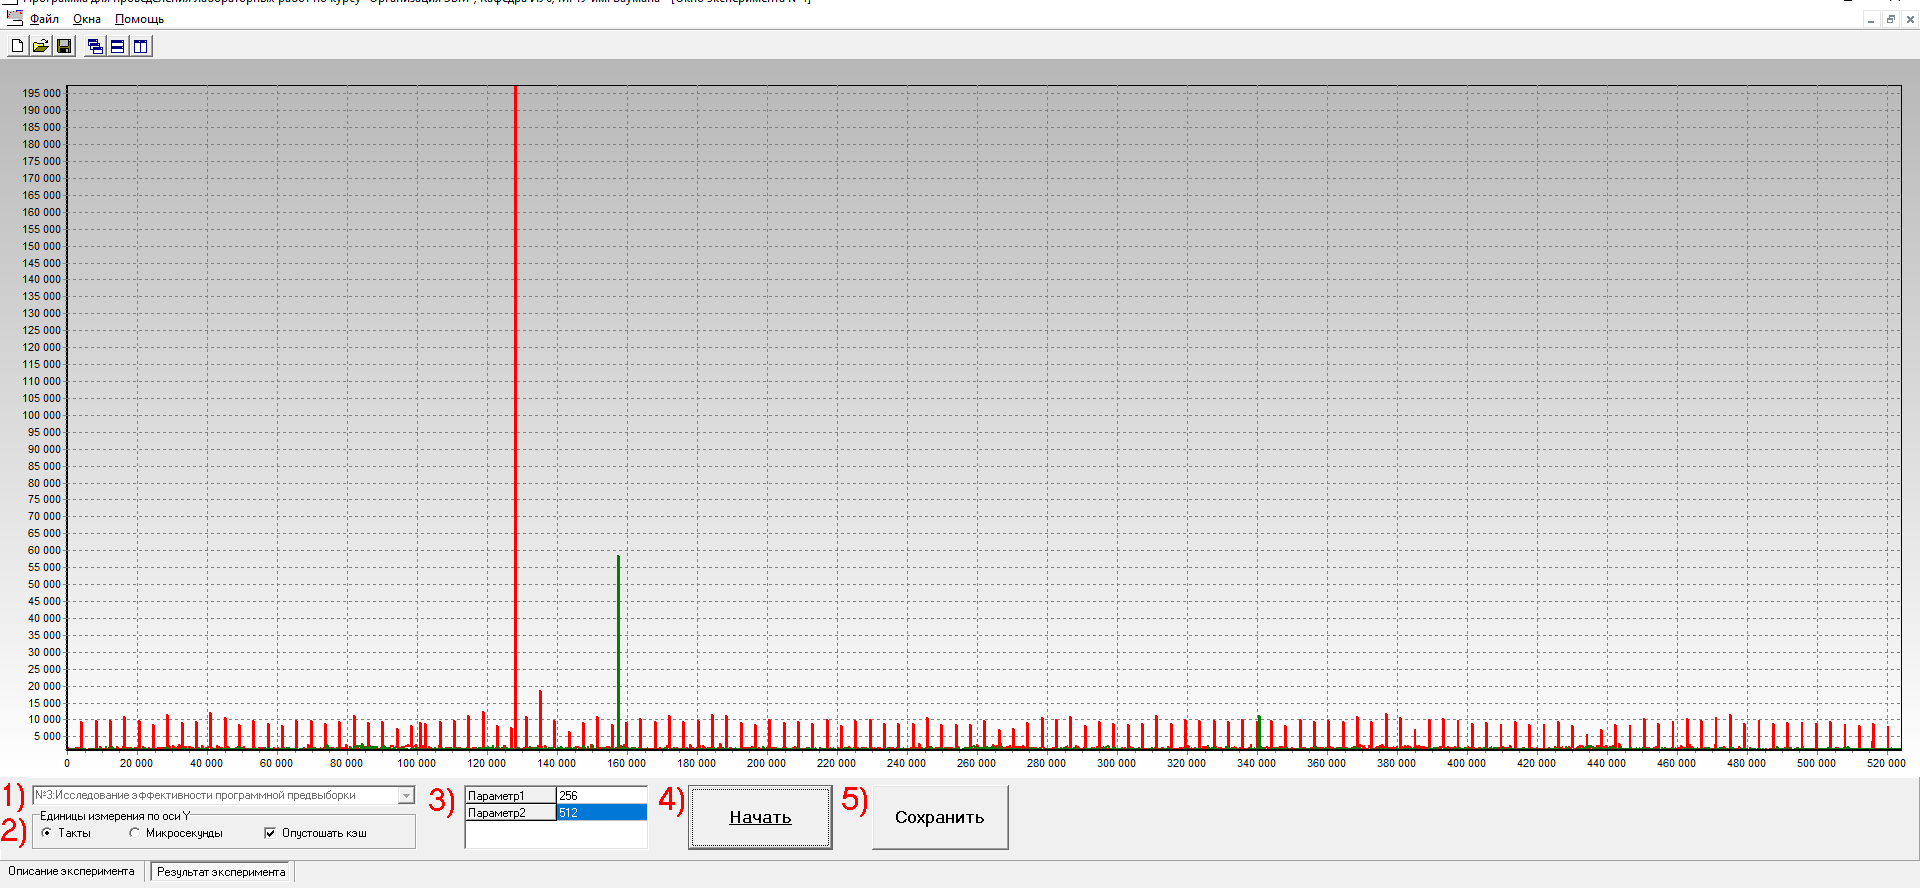
\includegraphics[width=170mm]{./img/3.png}
    \caption{Эксперимент 3: Исследование эффективности программной предвыборки}
\end{figure}

\begin{figure}[ht!]
    \centering
    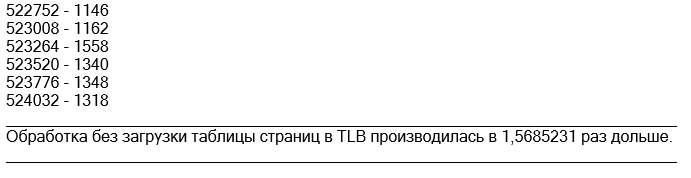
\includegraphics[width=100mm]{./img/03.png}
    \caption{Эксперимент 3: Результаты}
    \label{res_03}
\end{figure}

Как видно на рисунке \ref{res_03}, обработка без загрузки таблицы страниц в TLB производилась примерно в 1,6 раза дольше.

\section{Вывод}
При использовании предвыборки возможно значительное сокращение времени работы программы, практически вдвое, благодаря предварительной загрузке страниц в память.